\documentclass[portrait,a0,final] {a0poster} %\documentclass[a0,portrait] {a0poster}
\usepackage{multicol} 			%multi-column layout
\usepackage[left=2cm,right=2cm,bottom=0cm,top=0cm]{geometry}			%Reset margins
\usepackage{mathpazo}			%Load palatino font & pazo math
\usepackage{color}				%Needed for colour boxes & coloured text
\usepackage{amsmath}
\usepackage{graphicx}
% \usepackage{natbib}

\let\OLDthebibliography\thebibliography
\renewcommand\thebibliography[1]{
  \OLDthebibliography{#1}
  \setlength{\parskip}{0pt}
  \setlength{\itemsep}{0pt plus 0.3ex}
}

\setlength\parindent{0pt}

%%%Define colours and lengths
\definecolor{headingcol}{rgb}{1,1,1}			%Colour of main title
\definecolor{boxcol}{rgb}{0.7,0.2,0.2}		%Edge-colour of box and top banner
\fboxsep=1cm							%Padding between box and text
\setlength{\columnsep}{2cm}				%Set spacing between columns

%%%Format title
\makeatletter							%Needed to include code in main file
\renewcommand\@maketitle{%
\null									%Sets position marker
{
\color{headingcol}\sffamily\VERYHuge		%Set title font and colour
\@title \par}%
\vskip 0.6em%
{
\color{white}\sffamily\large				%Set author font and colour
\lineskip .5em%
\begin{tabular}[t]{l}%
\@author
\end{tabular}\par}%
\vskip 1cm
\par
}
\makeatother

\title{Climate change decouples drought from \\early winegrape harvests in France}

\author{Benjamin I. Cook\(^{1,2}\) \& Elizabeth M. Wolkovich\(^{3, 4}\)* \\ $^{1}$NASA Goddard Institute for Space Studies, New York, New York, $^{2}$Ocean and Climate Physics, Lamont-Doherty Earth Observatory, Palisades, New York\\$^{3}$Arnold Arboretum, Boston, Massachusetts, $^{4}$Organismic \& Evolutionary Biology, Harvard University, Cambridge, Massachusetts. *Presenting author}

\begin{document}

\hspace{-3cm}								%Align with edge of page, not margin
\colorbox{boxcol}{							%Coloured banner across top
\begin{minipage}{841mm}					%Minipage for title contents
\begin{center}
\maketitle
\end{center}
\end{minipage}}
\vspace{1cm}

\begin{multicols}{2}							%Use 3-column layout
\raggedcolumns

% \section*{Abstract}Climate change has altered the timing of winegrape harvests. Across France and globally grapes mature earlier by days and weeks compared to several decades ago \citep{Duchene:2005bd,Seguin2005,webb2011}. Understanding ties between climate change and these earlier harvests requires teasing out the often intertwined drivers of fruit maturation: temperature and drought in a longer-term context that includes data both before and after the start of anthropogenic shifts in the climate system. Here, we combine historical GHD records from across Western Europe \citep{daux2012} with independent reconstructions of temperature \citep{Luterbacher2004} and drought \citep{CookOWDA2015,Pauling2006} to investigate the climatic controls of early harvest dates from 1600--2007. We demonstrate that high temperatures and drought during the late spring and early summer (May-June-July) are the primary drivers of early harvests, but that in recent decades (1981--2007) drought has become largely decoupled from harvest timing. This decoupling is likely related to a decoupling of the climate itself: before significant anthropogenic warming high summer temperatures---that could speed fruit maturation---generally required drought conditions, on contrast recent higher temperatures often occur without drought conditions. Our results suggest climate change may have fundamentally altered the drivers of early winegrape harvests across France.

\section*{Introduction}

Warming trends in the earth's climate have advanced winegrape harvest dates in recent decades \cite{Duchene:2005bd,Seguin2005,schultzjones,webb2012}, with concomitant shifts in metrics tied to wine quality \cite{jones2005}. Both temperature and precipitation influence winegrape phenology with warmer temperatures generally accelerating grape vine  phenological development from flowering to fruit maturation and harvest, while increased precipitation tends to delay these events. An ideal harvest is typically favored by warm summers with above average early-season rains---ensuring the vines have sufficient heat and moisture to grow and mature early on---followed by dry conditions later in the year that shift vines towards investment in fruit production mid-season \cite{baciocco2014}. Despite much research, however, there have been few efforts to examine how consistently climate affects grape harvest dates over time.\\

Here, we analyze over 400 years (1600--2007) of winegrape phenology records from Western Europe \cite{daux2012} and over 100 years of wine quality estimates \cite{Broadbent2002}, comparing against both instrumental climate data for the 20\textsuperscript{th} century \cite{Harris2014} and proxy based reconstructions over the last 400 years of temperature \cite{Luterbacher2004}, precipitation \cite{Pauling2006}, and an index of soil moisture, the Palmer Drought Severity Index \cite{CookOWDA2015} (PDSI).\\

\begin{center}
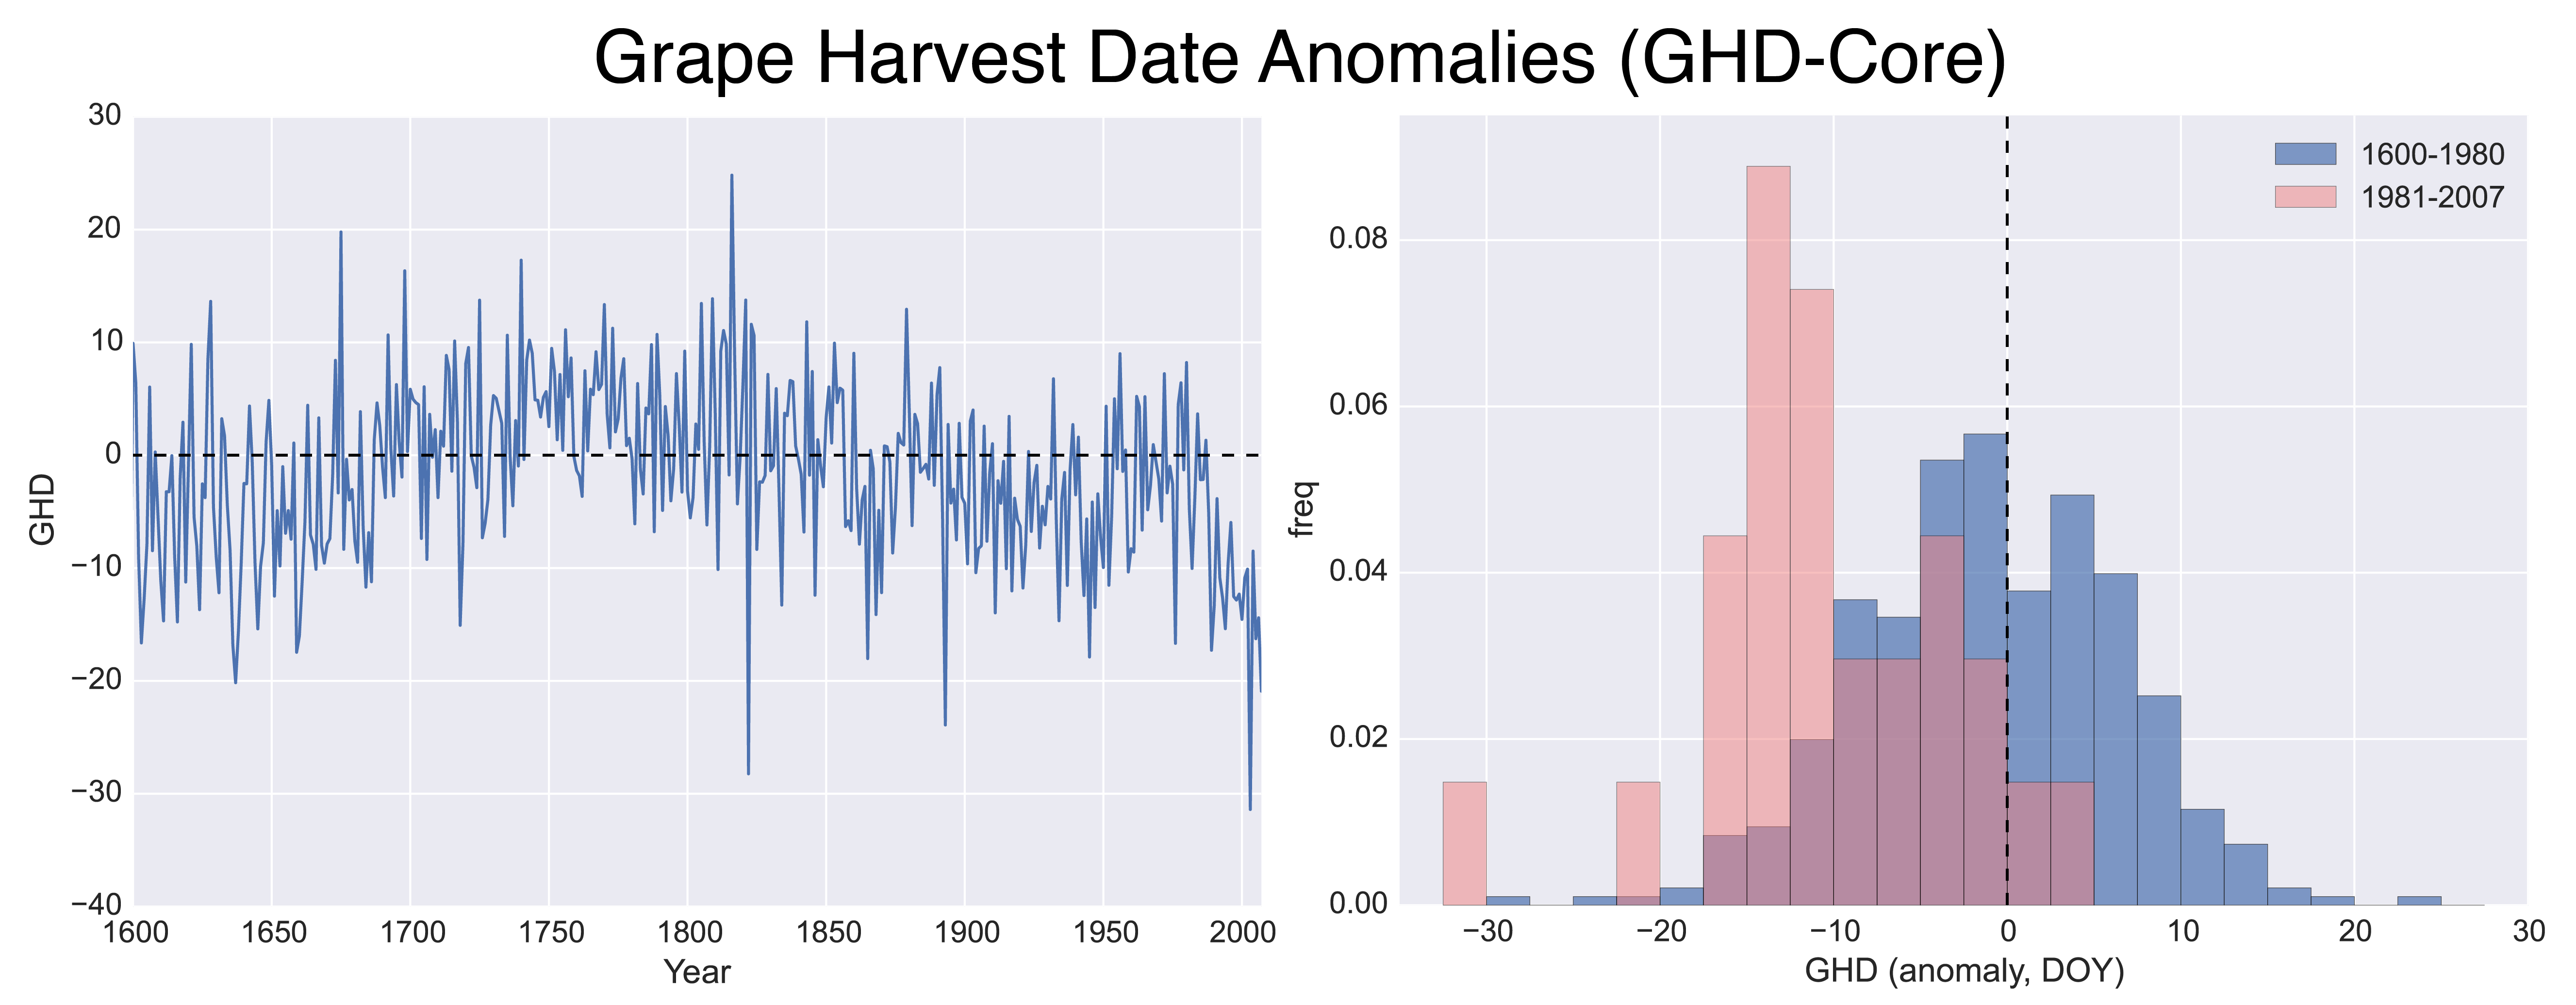
\includegraphics[width=0.4\textwidth]{../MANUSCRIPT/fig_01_time_ghd_core.png}
% \caption{Left panel: time series of Grape Harvest Date (GHD) anomalies from GHD-Core, composited from the Als, Bor, Bur, Cha1, LLV, SRv, and SWi regional GHD time series in DAUX. All anomalies are in units of day of year, relative to the average date calculated from 1600--1900. Right panel: normalized histograms of GHD anomalies (day of year) from GHD-Core for two periods: 1600--1980 and 1981--2007.}
\end{center}
From the GHD database of Daux et al 2012 \cite{daux2012}, we constructed a multi-site GHD index (GHD-Core) by averaging harvest date anomalies from 7 individual sites across France and Switzerland. This series (\emph{above, left panel}) shows the latest GHD anomaly in the record at 1816, the so called `Year without a Summer' following the eruption of Mount Tambora in Indonesia. The earliest date in the record is 2003 (-33.4 days early), coinciding with one of the worst summer droughts and heat waves in recent history. During the last several decades of the record (1981--2007) there has been a strong shift towards earlier harvest dates, on average -10.6 days earlier (\emph{above, right panel}). 
\section*{Results}
\begin{center}
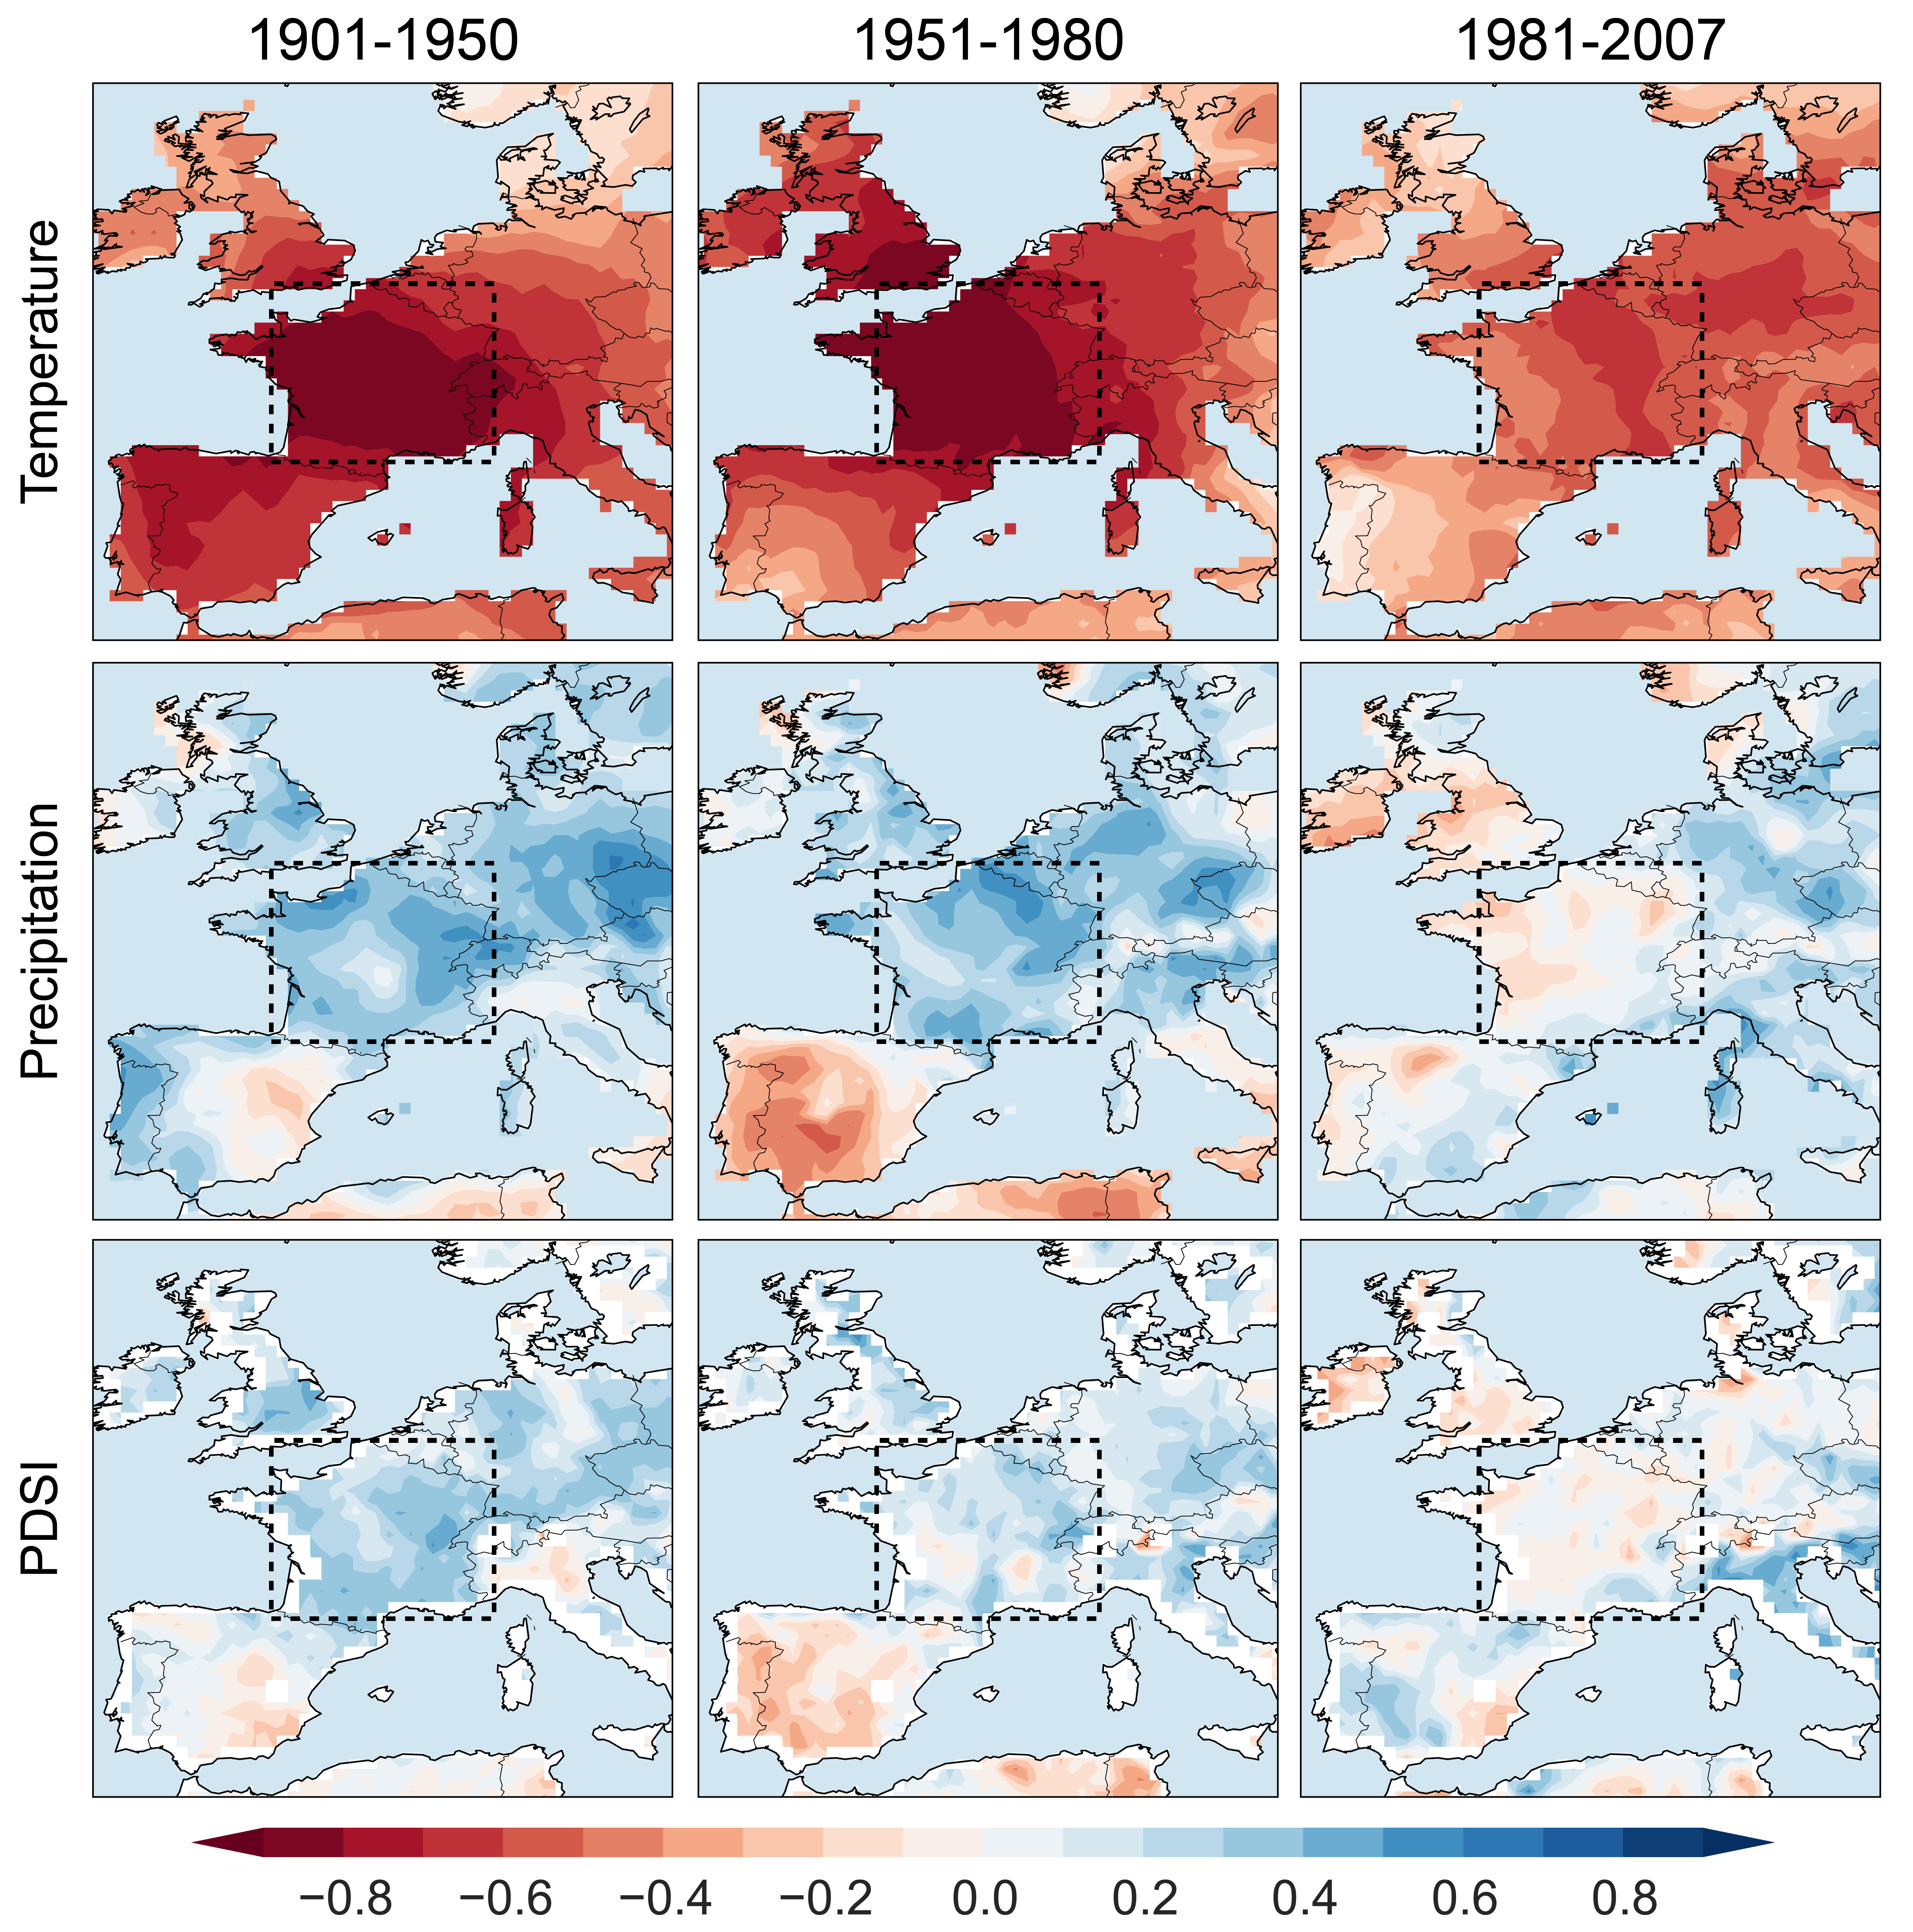
\includegraphics[width=0.35\textwidth]{../MANUSCRIPT/fig_02_core_cru_MJJ.png}
\end{center}
\vspace{1ex}
\emph{Above:} Point-by-point correlations (Spearman's rank) between GHD-Core and May-June-July (MJJ) temperature, precipitation, and Palmer Drought Severity Index (PDSI) for three periods. MJJ temperatures were the best predictor of GHD-Core anomalies and showed a consistent relationship across time ($6-7$ days advancement per $^{\circ}C$). In contrast, both PDSI and precipitation are positively correlated with GHDs from 1901--1980, indicating below average precipitation and drought conditions during MJJ will lead to earlier harvests, but since 1981 the relationship between GHD and these moisture variables has become insignificant (\emph{see above}). 
\begin{center}
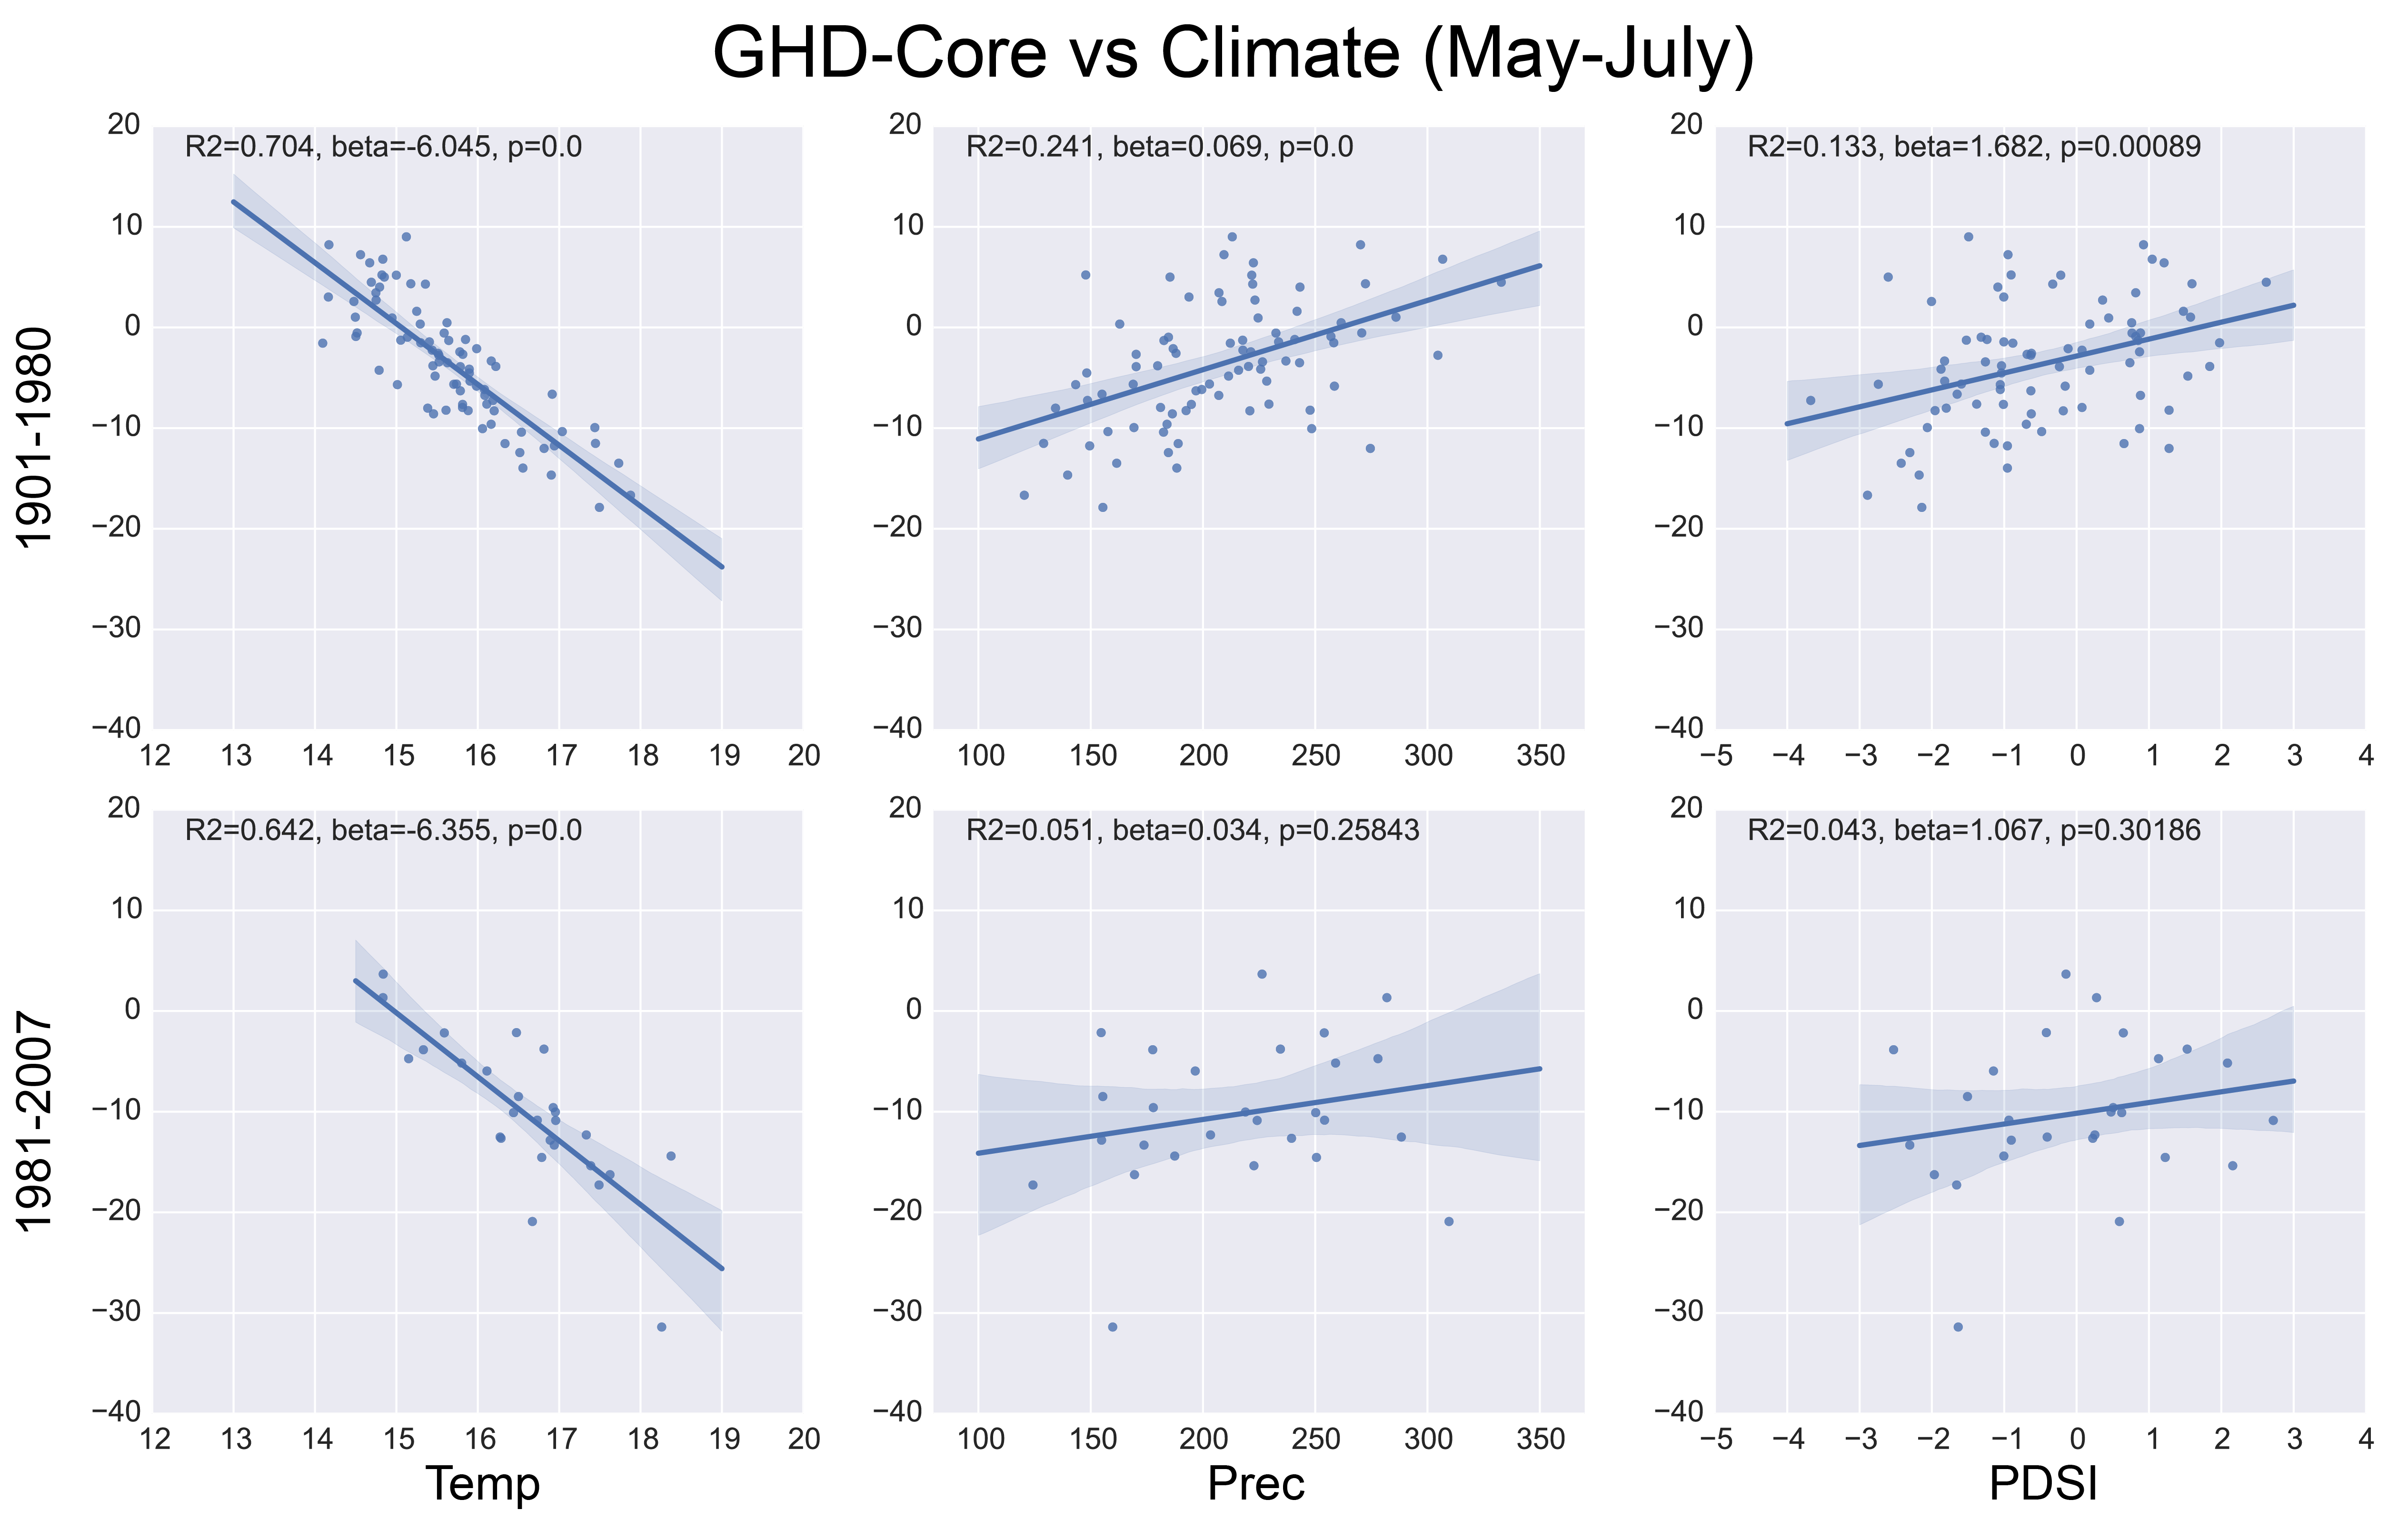
\includegraphics[width=0.3\textwidth]{../MANUSCRIPT/fig_03_MJJ_clim_regplots.png}
\end{center}
\vspace{1ex}
\emph{Above:} Linear regressions between GHD-Core and May-June-July climate variables from CRU 3.21, averaged over the main GHD-Core region, across two time periods: 1901-1980 and 1981-2007.\\

\columnbreak
To further explore this, we calculated composite average climate anomaly maps (\emph{below}) from the climate reconstructions for years when GHD occurred -7.8 days early or earlier (one SD). 
\vspace{2ex}
\begin{center}
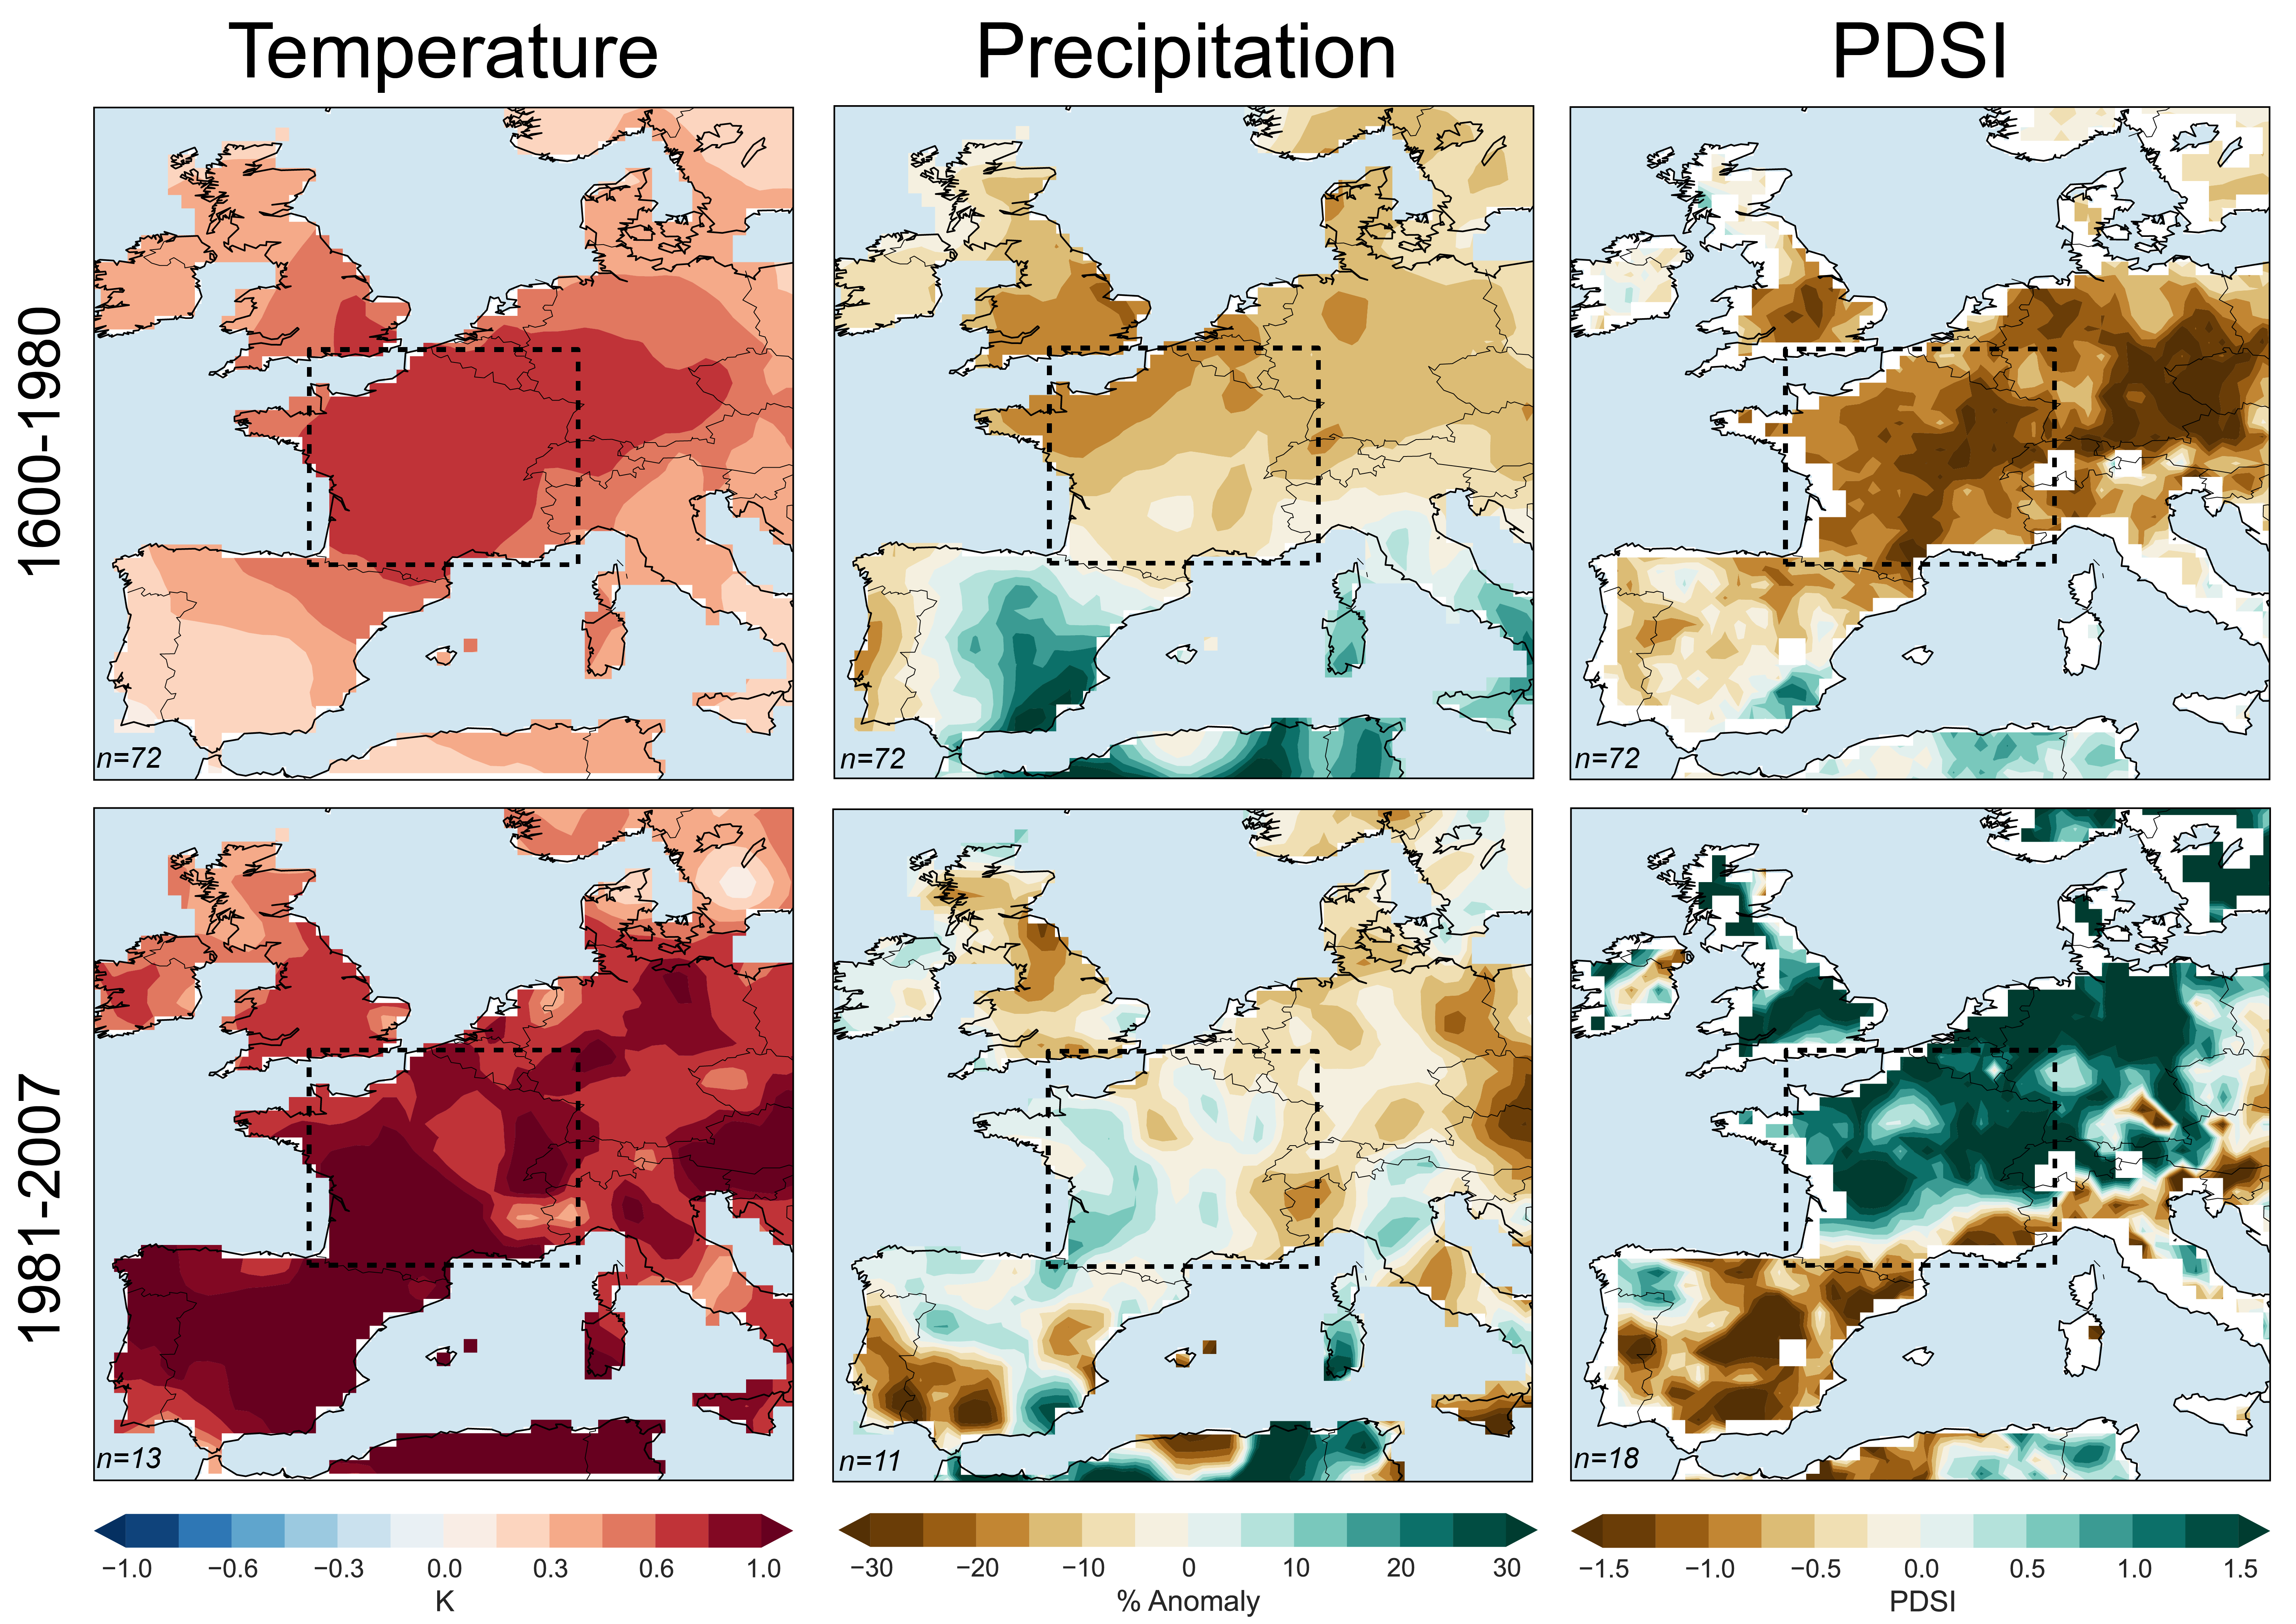
\includegraphics[width=0.45\textwidth]{../MANUSCRIPT/fig_04_comp_map_JJA_comp.png}
\end{center}
\vspace{1ex}
\emph{Above:} Composite temperature, precipitation, and PDSI anomalies from the various climate reconstructions, for years with early harvest dates ($\le-7.8$ days early). Early harvests are associated with warmer than average conditions in both intervals, increasing in intensity in the more recent period, consistent with large-scale warming trends over Europe. In contrast, the typical dry anomalies associated with early harvests from 1600--1980 effectively disappear in the more recent interval.\\

\indent As harvest dates are generally coupled to wine quality in France we tested for shifting relationships between wine quality in Bordeaux and Burgundy and climate from 1900-1980 and 1981-2001 (below). Results considering wine quality and climate in many ways recapitulated our findings above.\\


\emph{Below:} Coefficients and p-values from ordered logit models of wine quality data (on a scale of 0 to 5) and grape harvest dates (GHD) and Luterbacher May-June-July seasonal temperatures for the periods 1900-1980 and 1981-2001. Higher temperatures and lower amounts of precipitation yield higher odds of a high quality wine and these relationships were generally consistent across regions and before and after 1980 (though note red wines in Burgundy after 1980). 
\begin{center}
\begin{tabular}{||r||l|l||l|l||}
  \hline
 & GHD: 1900-1980 & GHD: 1981-2001 & Temp: 1900-1980 & Temp: 1981-2001 \\ 
  \hline
Red Bordeaux & -0.117 ($<$0.01) & -0.133 (0.03) & 1.244 ($<$0.01) & 1.308 (0.01) \\ 
  White Bordeaux & -0.084 ($<$0.01) & -0.079 (0.14) & 0.951 ($<$0.01) & 1.109 (0.02) \\ 
  Red Burgundy & -0.102 ($<$0.01) & -0.101 (0.18) & 0.403 (0.06) & 0.612 (0.23) \\ 
  White Burgundy & -0.093 (0.02) & -0.144 (0.07) & 0.564 (0.04) & 1.262 (0.03) \\ 
   \hline
\end{tabular}
\end{center}
Lower soil moisture also increased the odds of a higher quality vintage, however---in line with our findings above---this was seen only before 1980. After 1980, in both Bordeaux and Burgundy significant relationships between quality and PDSI disappeared and the magnitudes decreased greatly.
\begin{center}
\begin{tabular}{||r||l|l||l|l||}
  \hline
 & Prec: 1900-1980 & Prec: 1981-2001 & PDSI: 1900-1980 & PDSI: 1981-2001 \\ 
  \hline
Red Bordeaux & -0.013 ($<$0.01) & -0.011 (0.12) & -0.457 ($<$0.01) & -0.119 (0.61) \\ 
  White Bordeaux & -0.014 ($<$0.01) & -0.014 (0.06) & -0.291 (0.02) & -0.234 (0.32) \\ 
  Red Burgundy & -0.018 ($<$0.01) & 0 (0.96) & -0.273 (0.03) & 0.12 (0.64) \\ 
  White Burgundy & -0.011 (0.05) & -0.013 (0.08) & -0.101 (0.52) & -0.199 (0.41) \\ 
   \hline
\end{tabular}
\end{center}

\section*{Conclusions}
Our results show that high temperatures and drought during the late spring and early summer (May-June-July) are the primary drivers of early harvests, but that in recent decades (1981--2007) drought has become largely decoupled from harvest timing. This decoupling is likely related to a decoupling of the climate itself: before significant anthropogenic warming high summer temperatures---that could speed fruit maturation---generally required drought conditions. When soils are dry, surface energy partitioning favors sensible over latent (evapotranspiration) heating, increasing soil and air temperatures. Western Europe is a region where this feedback is thought to be especially strong, however, with climate change higher temperatures often occur without drought conditions.\\ 

Our results are consistent when including multiple sites, but some regions do deviate from overall responses. This is not unexpected as regions grow different varieties, have experienced different magnitudes of climate change and have varying local climates. We expect that local effects of drought and soil moisture on winegrape harvest timing and quality are still important drivers, but our results suggest large-scale relationships with drought have been decoupled by climate change. \\

\emph{Acknowledgements:} V. Daux and co-authors for data, in particular thanks to I. Garcia de Cortazar for help with the Daux data, H. Eyster, S. Gee \& J. Samaha for extracting wine quality data.\\

\bibliographystyle{/Users/Lizzie/Documents/EndnoteRelated/Bibtex/styles/science.bst}
{\def\section*#1{}
\bibliography{/Users/Lizzie/Documents/EndnoteRelated/Bibtex/LizzieMainMinimal}
}

\end{multicols}
\end{document}


% Show figures
% Show quality tables

\begin{figure}

\end{figure}

\begin{figure}

\end{figure}

%%
%% General
%%


This may be due to direct drought impacts on fruit maturation by increasing abscisic acid production\cite{webb2012}, but may also arise indirectly via feedbacks between soil moisture and air temperature. 

This decoupling is likely related to a decoupling of the climate itself: before significant anthropogenic warming high summer temperatures---that could speed fruit maturation---generally required drought conditions, on contrast recent higher temperatures often occur without drought conditions. 


%%
%% Methods
%% 

% Data: Climate Data and Reconstructions.
\noindent Instrumental temperature and precipitation data for the twentieth century (1901--2012) are taken directly from version 3.21 of the CRU climate grids\cite{Harris2014}.We also use a drought index, an updated version of the Palmer Drought Severity Index (PDSI\cite{Palmer:1965}) derived from the CRU data\cite{Schrier2013}. PDSI is a locally standardized indicator of soil moisture, calculated from inputs of precipitation and evapotranspiration. PDSI integrates precipitation over multiple months and seasons (about 12 months), and so it incorporates longer term changes in moisture balance beyond the immediate months or season.\\
\indent To extend our analysis further back in time, we also used three largely independent proxy based reconstructions of temperature\cite{Luterbacher2004}, precipitation\cite{Pauling2006}, and PDSI\cite{CookOWDA2015}. The temperature and precipitation products are 3-month seasonal reconstructions (DJF, MAM, JJA, SON) using primarily historical documentary evidence over the last 500 years. The temperature reconstruction covers the period 1500--2002; the precipitation reconstruction covers 1500--2000. The PDSI reconstruction is summer season only (JJA) and is based entirely upon tree ring chronologies distributed across Europe. It covers the entire Common Era, up through 2012. Prior to comparisons with the GHD data, we anomalized all three reconstruction products to a zero mean over 1600--1900, the same baseline period used in the GHD data.